\chapter{Introduction}
\label{ch:intro}
This chapter provides an overview of steganography in general and image steganography in particular. The use of digital image steganography as a covert communication medium is also discussed. An explanation of terminology used throughout the document are listed at the end of this chapter. 
\section{Background}
The use of steganographic techniques to hide messages in everyday objects is thought to have existed for thousands of years. The Greek historian Herodotus tells the story of Demeratus who wanted to inform his friends in Greece of an impending Persian invasion  \cite{kahn1996history}. Demeratus is said to have concealed the message in writing tablets in such a way that, to the casual observer, appeared to be blank tablets covered with wax. The hidden message was inscribed on the wooden tablet itself and was recovered by the recipients after melting the wax covering it. 
Contemporary methods of digital steganography, on the other hand, make subtle modifications to bits that constitute digital files to hide messages in plain sight  \cite{hinson2009introduction}.  Such modifications are subtle in that they are not readily noticeable to the casual observer.   Similar methods can also be applied to other digital mediums like video \cite{crawford2010supraliminal} and audio. If the message to be hidden is relatively short in comparison to the size of the file, this encoding ensures that the original and modified files appear exactly the same to the casual observer.
%Steg image
\begin{figure}[h!]
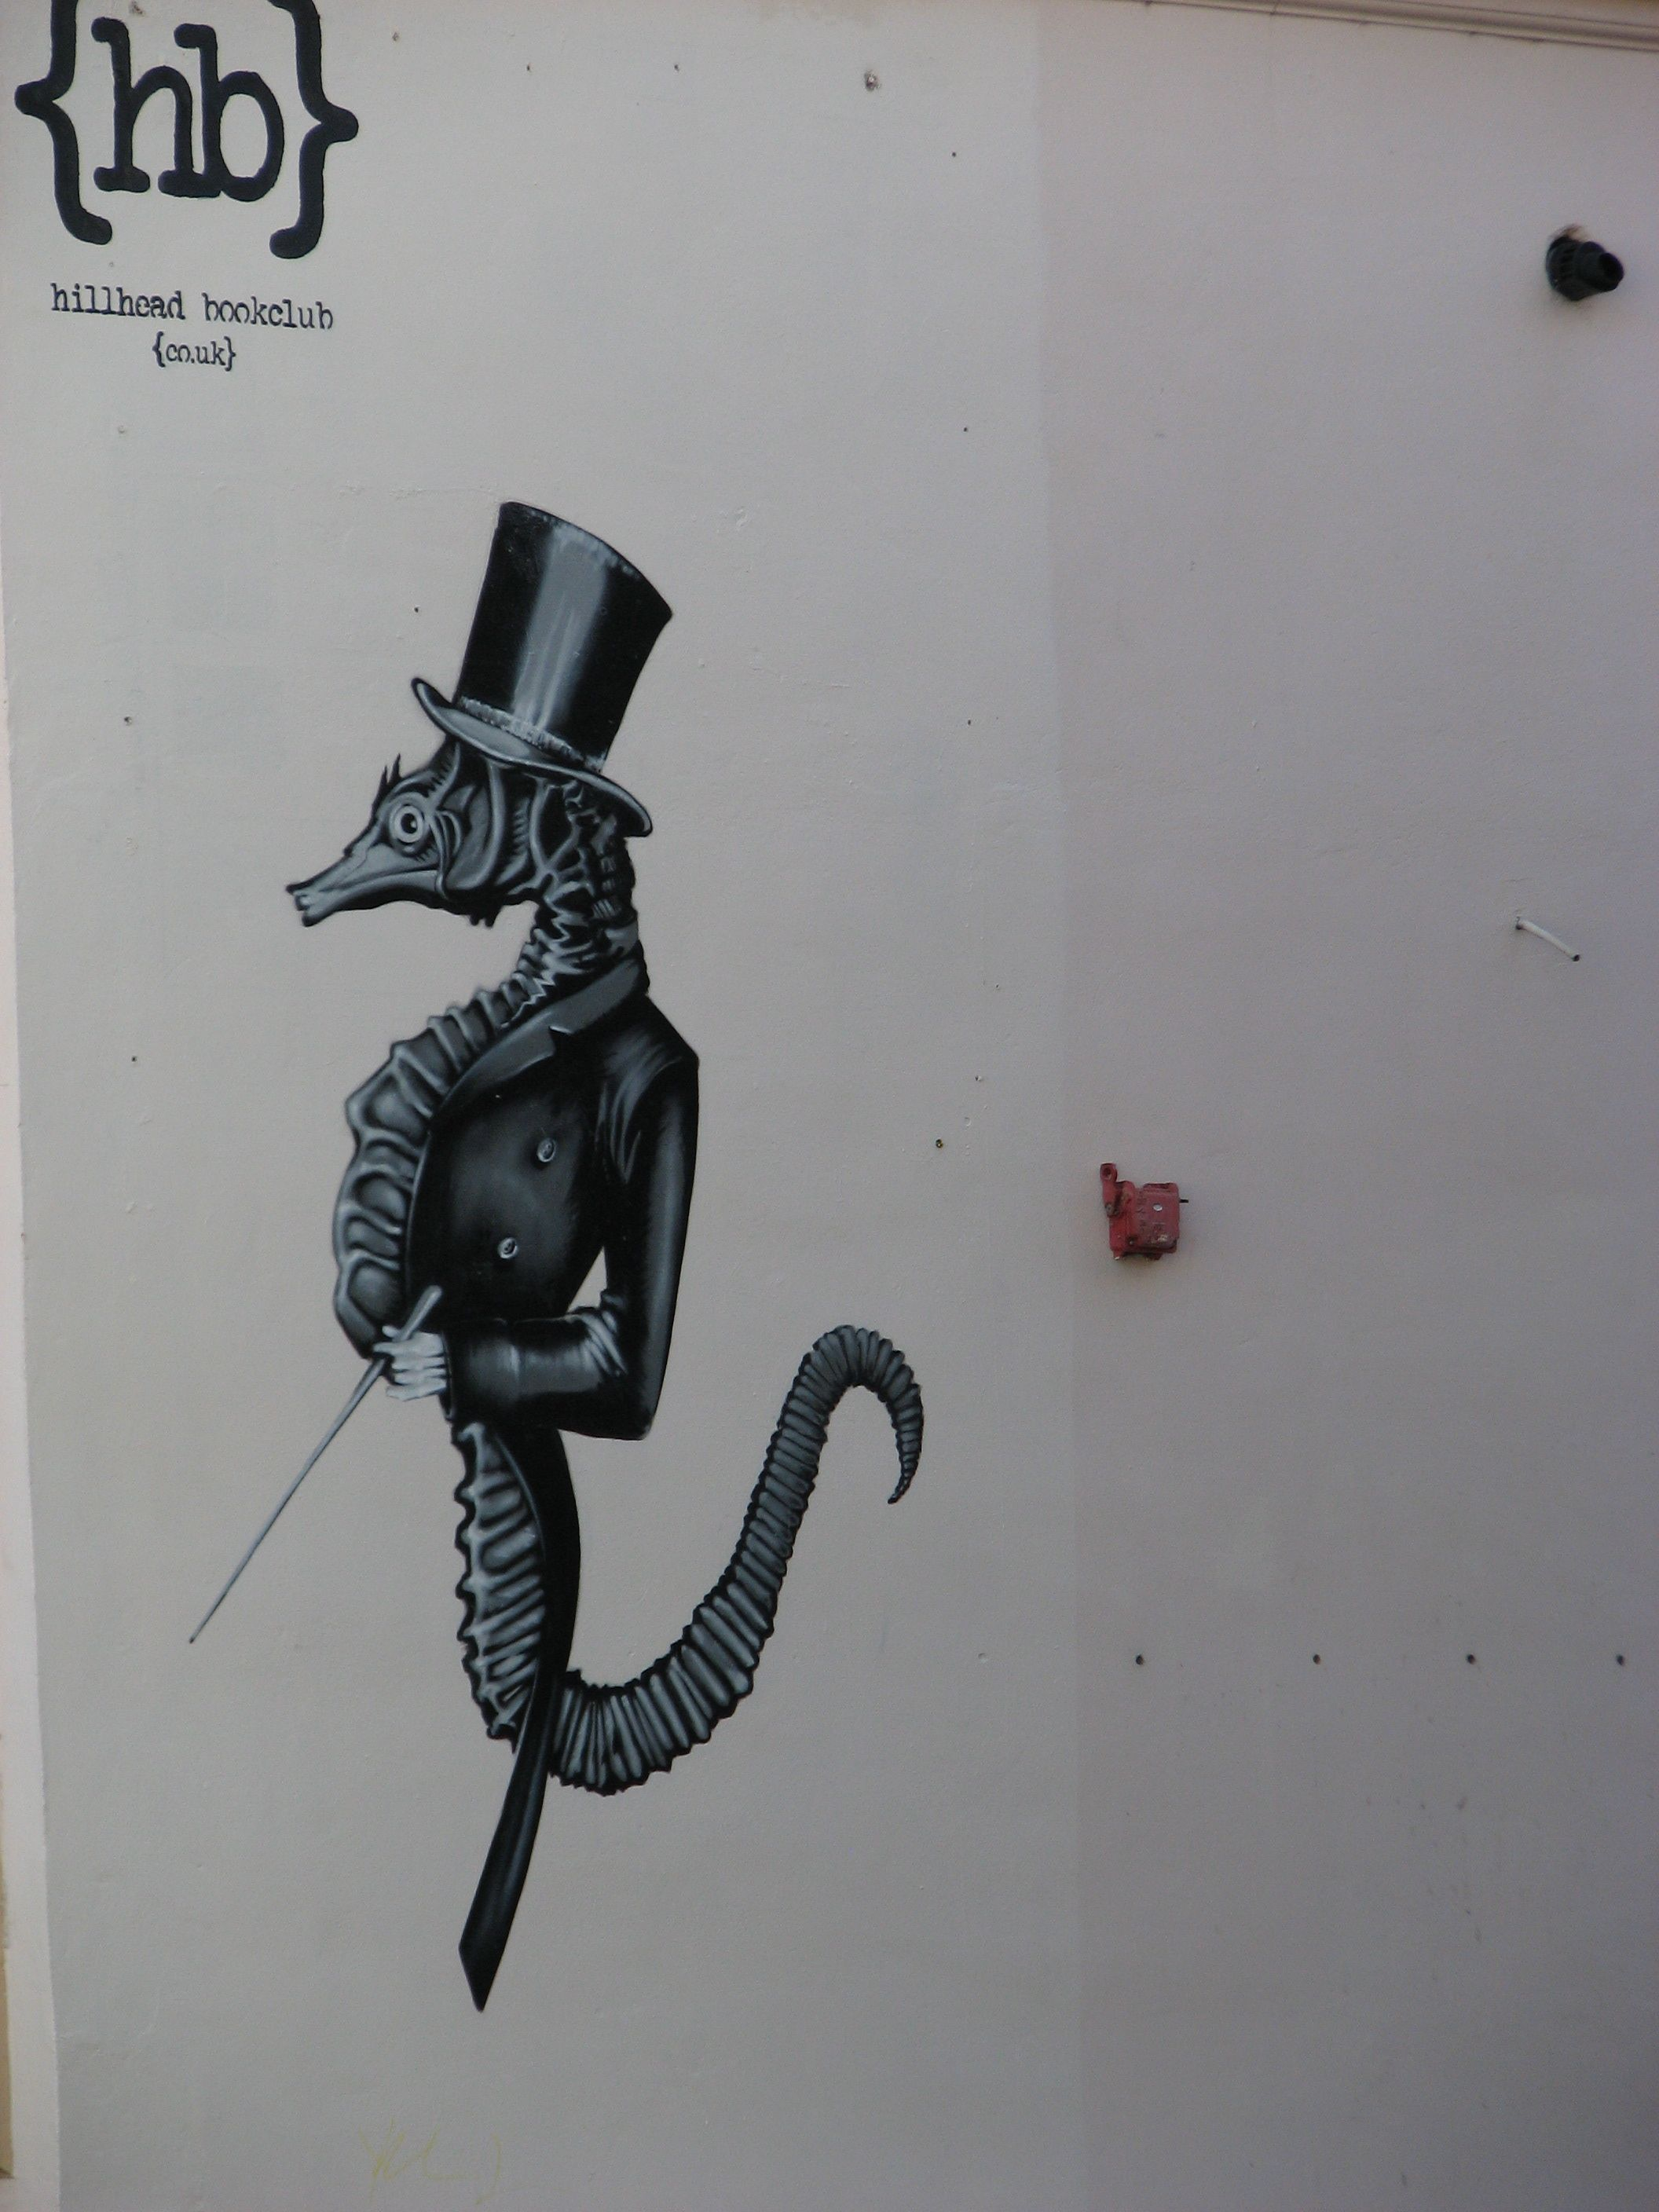
\includegraphics[scale=0.10]{hb1}
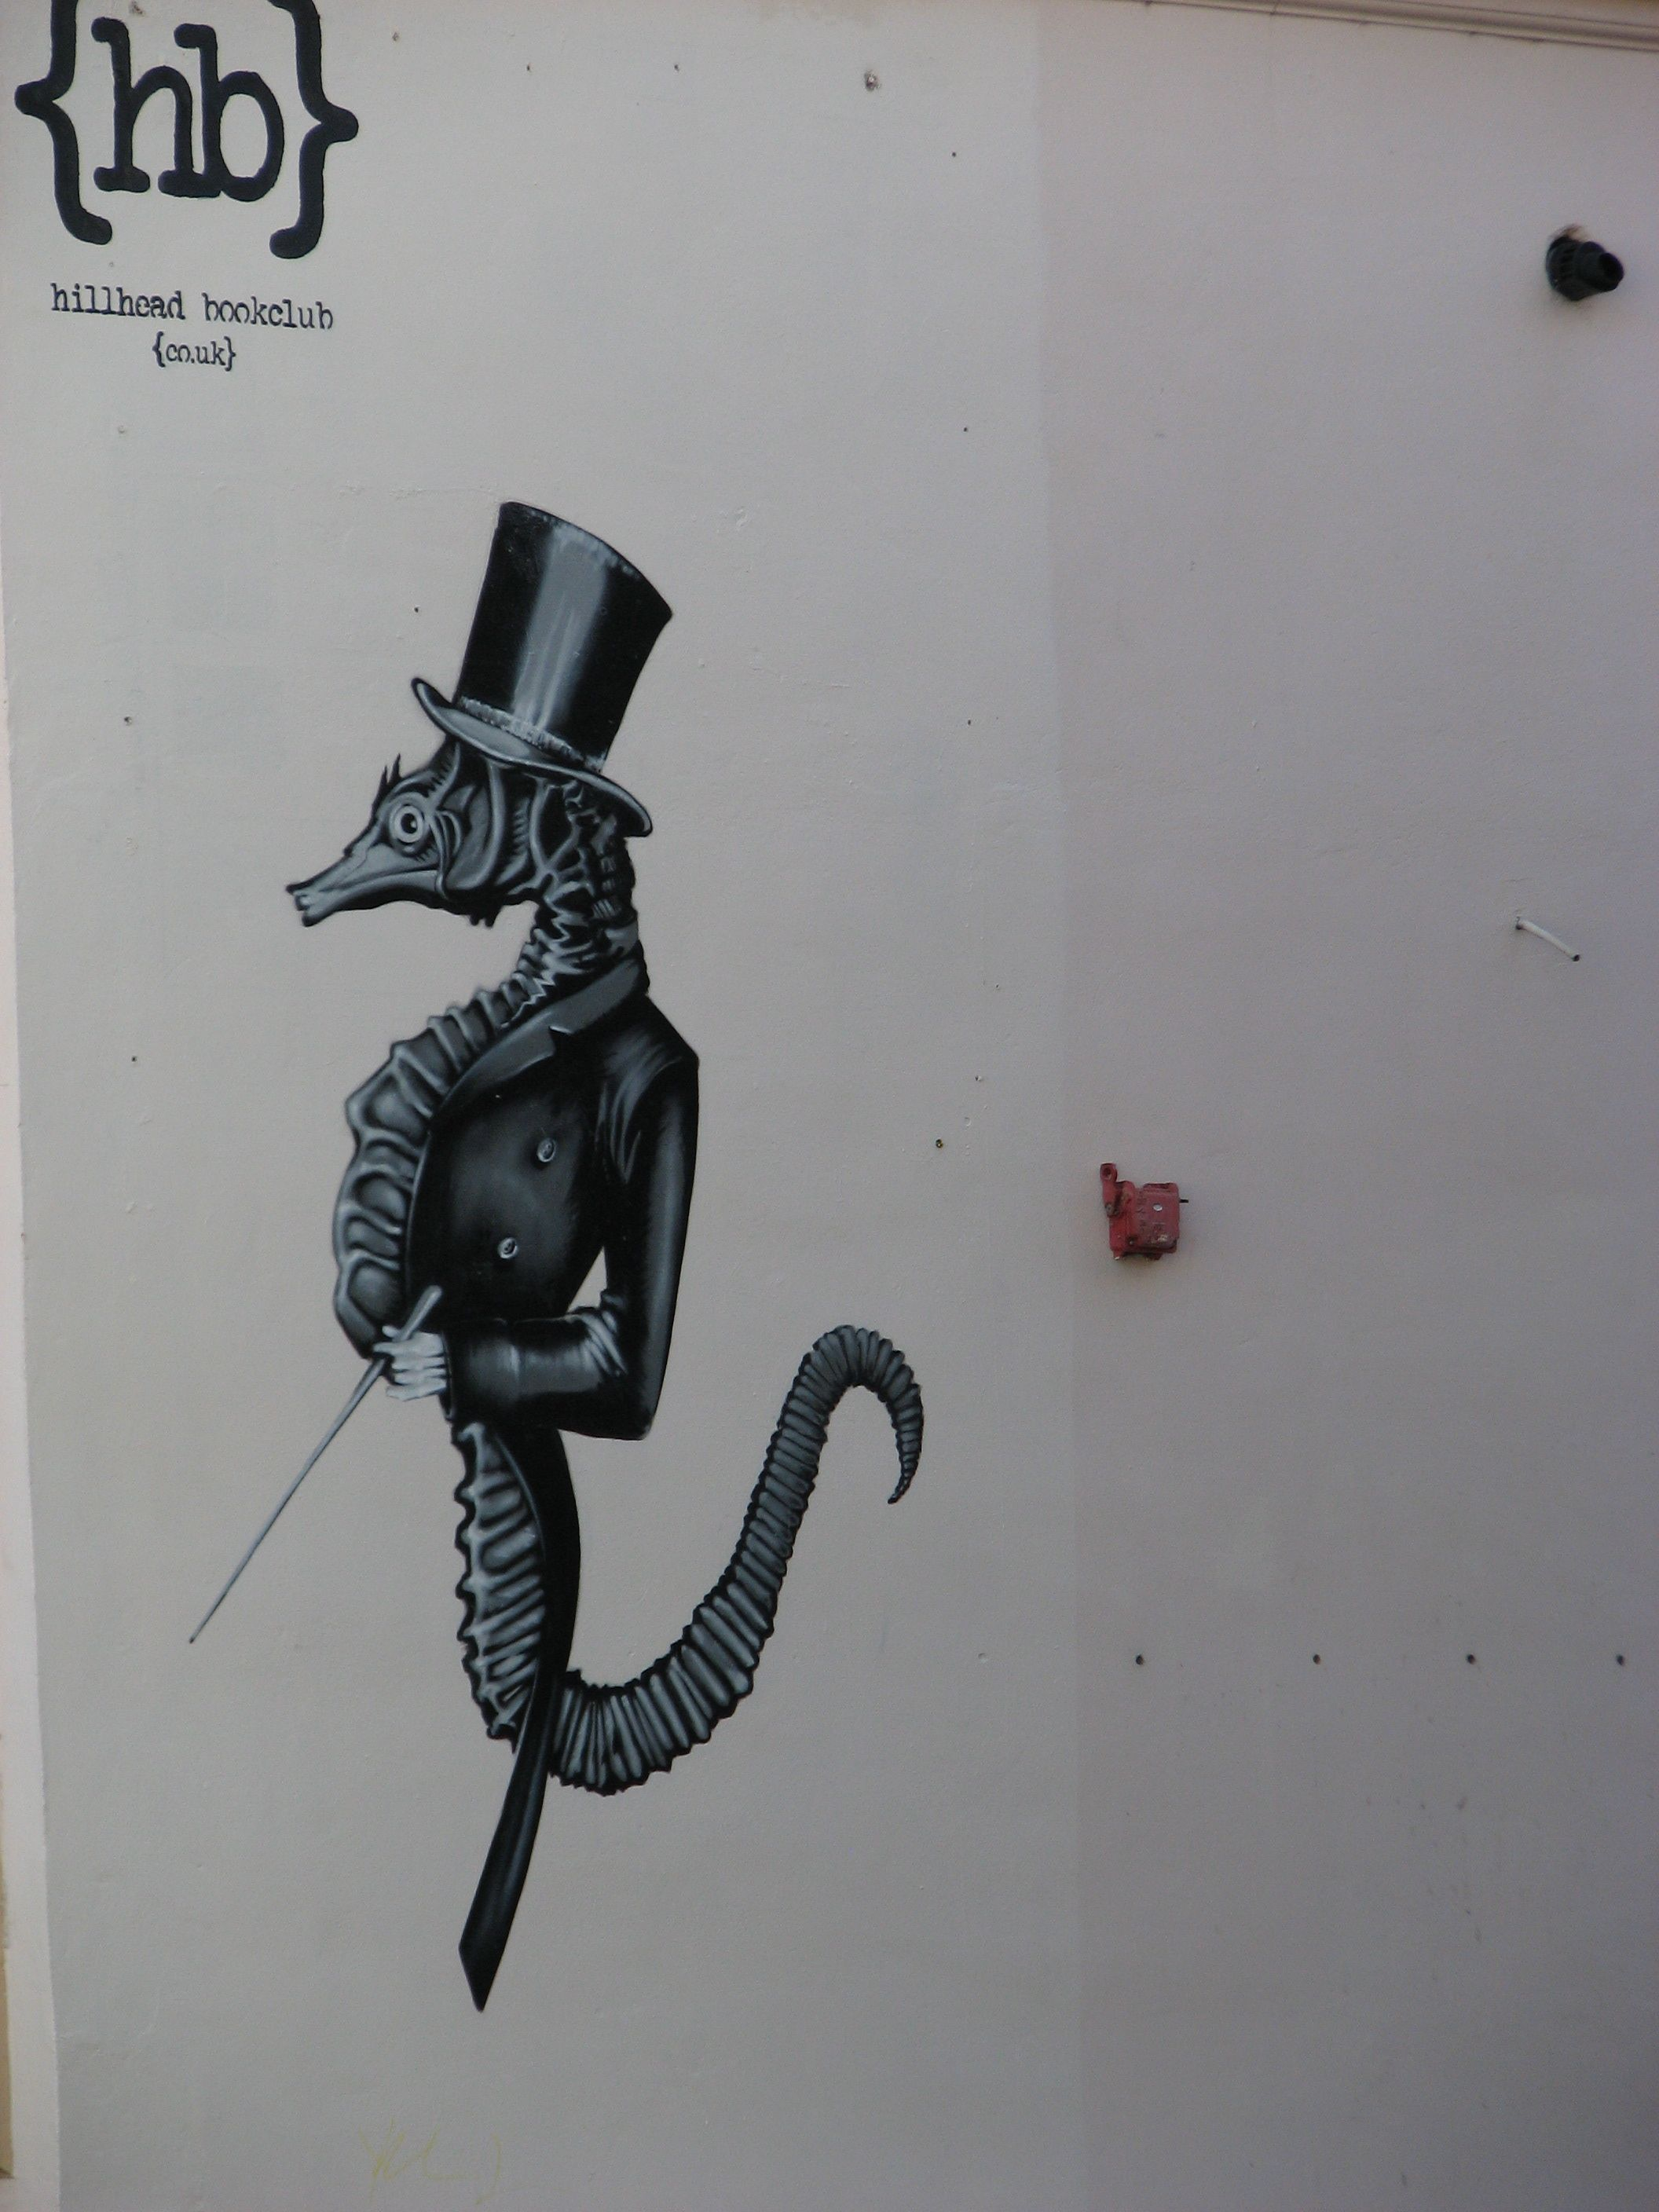
\includegraphics[scale=0.10]{hb1}
\caption{\emph{The images above show that there are no obvious differences between an unaltered image and the same image with data embedded in it using open source steganographic software called Stepic \cite{stepnic}. The image on the right contains the following text embedded using steganography : ``Thoughts, words, and deeds, the statute blames with reason;  But surely dreams were ne'er indicted treason \cite{burns}"}}
\label{fig:stegexample}
\end{figure} 
%Steg image
Colour images, for example, can use anywhere between 4 to 8 bits of data to represent one colour value of a pixel (either red, green or blue). A change to a single bit for each colour would still ensure that the image resembled the original \emph{See: Figure \ref{fig:stegexample}}.
Image steganography is perhaps the most popular used form of digital steganography as a large number of freely available tools that allow one to embed data in images are easily available. These tools, described in more detail in Chapter \ref{ch:litsurvey} allow for embedding data in almost any image format. Some of these tools also provide encryption using a password derived key to provide an additional layer of security to the embedded data. The hidden message can then be recovered by the recipient with a suitable decoding tool and the correct password or decryption key. This makes image steganography a viable medium for covert communication.  
Another interesting use of image steganography is for the purposes of copyright enforcement  \cite{kundur2002digital}. By using digital watermarks that contain copyright information,  it is possible to uniquely identify an image even after it has  been modified. These ``marks'' can be read by specialised software which can determine the original source of the image. 
\par The use of image steganography as a covert communication channel on the internet has always been a contentious topic and a source for much speculation. Analysis of a terrorist user manual, the Technical Mujahid \cite{alfajr}, by the United States Central Intelligence Agency (CIA) mentioned chapters in that outline various concealment techniques utilising image steganography. The manual describes the use of steganography as an additional layer of security for encrypted data. It's however, difficult to ascertain whether these techniques are in use in the wild. An argument for the limited use of steganography would be that steganography is an approach that relies on security through obscurity. Security through obscurity implies the use of a secret, but insecure, method of protecting a resource. An example of this would be hiding one's room keys under the doormat in the hope that a thief would never find it there. In 2000, Provos and Honeyman \cite{provos2001detecting}  carried out an analysis of images available on eBay for steganographic content.  They argue that either there isn't  significant use of steganography on the internet or that the steganographic techniques used are undetectable by the methods used by them. They also concede that it might be possible that encryption might have been used on the data embedded in the images and that they were unable to decrypt it. Their analysis is based on a fairly large (2 million) image dataset acquired from eBay.   More recent news reports  \cite{spies2010} suggest that members of a Russian spy ring arrested in the United States in 2010 used steganography to communicate with each other. Reports speculate that these individuals posted images with steganographic content on public image hosting sites with sensitive data embedded in them. The news reports, however, did not provide any technical details regarding the steganography methods used. This project attempts to revisit the seminal work conducted by Provos \emph{et al} to try and establish real world usage of steganography.

It would be trivial to prove the \emph{existence} of steganography if one were provided the unaltered host image along with the image carrying the steganographic payload. By calculating the binary difference of the steganographic image from the unaltered image, one could easily discover the payload embedded in the image. However, this is an unrealistic expectation as the steganographic host medium will be less likely to be found along with the altered copy. Hence it is necessary to user other means for the steganalysis of images that do not require the original host image for comparison.


\section{Terminology}
The following terms are used throughout the document to refer to various aspects of steganography. 
\begin{itemize}
\item{\emph{Steganogram:}} An \emph{portmanteau} of steganography and telegram, this is used to refer to an image containing steganographic content. The content could be text, images or audio. In this report, a steganogram is used to refer to an image containing hidden text.
\item{\emph{Stegnanalysis:}} The process of testing a digital artifact for embedded steganographic data. This analysis may be carried out either using statistical measures or by matching the contents of the digital artifacts against a database of known steganographic signatures.
\item{\emph{Cover medium:}} Any digital medium used as a host for hiding data. Throughout this document, the cover medium is used to refer to digital imagery.
\end{itemize}

